\documentclass[11pt,a4paper]{article}
\usepackage[T1]{fontenc}
\usepackage{lmodern}
\usepackage[margin=24mm]{geometry}
\usepackage{amsmath,amssymb,amsthm,booktabs,array,graphicx}
\usepackage{xcolor,microtype}
\usepackage[unicode,colorlinks=true,linkcolor=blue!45!black,urlcolor=blue!45!black,citecolor=blue!45!black]{hyperref}
\hypersetup{pdftitle={SRG Contribution Geometry: Exact Prefixes, Carry Lattices, and Neighboring-Pair Transformations},pdfauthor={Hilmir Frímann Halldórsson},pdfsubject={v0.1 manuscript and exact twelve-file candidate awaiting GPT review}}
\graphicspath{{../figures/}}
\newtheorem{theorem}{Theorem}[section]
\newtheorem{proposition}[theorem]{Proposition}
\newtheorem{corollary}[theorem]{Corollary}
\newcommand{\diag}{\operatorname{diag}}
\newcommand{\sech}{\operatorname{sech}}
\newcommand{\tr}{\mathrm T}
\newcommand{\N}{\mathbb N}
\setlength{\parindent}{0pt}
\setlength{\parskip}{5pt plus 1pt}
\setlength{\emergencystretch}{2em}

\newcommand{\beginwidepage}{\clearpage
\newgeometry{layoutwidth=297mm,layoutheight=210mm,left=18mm,right=18mm,top=16mm,bottom=18mm}
\special{papersize=297mm,210mm}}
\newcommand{\finishwidepage}{\clearpage\restoregeometry\special{papersize=210mm,297mm}}

\title{\Large SRG Contribution Geometry:\\Exact Prefixes, Carry Lattices,\\and Neighboring-Pair Transformations}
\author{Hilmir Frímann Halldórsson}
\date{v0.1 \quad 13 October 2026\\\small Manuscript and exact publication candidate awaiting GPT review}
\begin{document}
\maketitle
\begin{abstract}
The neighboring raw contributions $0.48$ and $0.508$ of the SRG master multiplication form a nearly balanced split diameter. Its circle provides a concrete starting point for studying decimal contribution layers. We prove when a raw layer becomes exactly independent of further input digits, how legal integer carries move a split on a fixed circle, and how reciprocal scaling instead preserves the pair product. Passing to the next overlapping pair obeys an exact scale-plus-reciprocal law, with a rational matrix and a telescoping logarithmic coordinate. We give complete proofs that $w_3=0.508$ is the unique largest full raw contribution and that positive canonical adjacent decimal contributions have normalized imbalance at least $1/19$. An accepted, certified finite scan through 64 input places supplies precisely delimited rankings, zero cases and sign comparisons. All factor-labelled inputs and exact tables accompany the proposed edition. These are results about multiplication and an explicitly adopted geometry of its summands; no physical dynamics is inferred.
\end{abstract}

\section{The two layers that start the construction}
\label{sec:start}
Begin with the actual weighted contributions
\begin{equation}
w_2=0.48=\frac{12}{25},\qquad
w_3=0.508=\frac{127}{250},\qquad
w_4=0.1704=\frac{213}{1250}.
\label{eq:threeweights}
\end{equation}
Picture multiplication as a stack of layers. Each layer collects digit products whose four indices add to that depth. Neighboring layers supply two lengths, which we place end to end along a circle's diameter. The depth labels remain attached; the stack is an arithmetic organization, not a physical clock or an assigned direction for each constant.

For depths 2 and 3 the diameter is $0.988$, the radius is $0.494$, and the split lies $0.014$ to the left of the center. The perpendicular height from that split to the upper semicircle is approximately $0.493801579584350864$. It almost reaches the radius because the two lengths are close. They are not equal.

The question is what persists when we supply more digits, carry value between layers, or move to the overlapping pair $(w_3,w_4)$. These three changes have different invariants. The paper develops the accepted PH04 analysis~\cite{ph04,review}; the earlier positive-factor construction~\cite{multiplication,ph03} supplies geometry, while the use of neighboring \emph{summands} is the declared new representation.

\clearpage
\subsection{A circle, its inverse, and the information in its scale}
\label{sec:circle}
For $a,b>0$, use diameter endpoints $(-R,0),(R,0)$ and split point $(X,0)$, so the left and right segments are $a=R+X$ and $b=R-X$. The upper-circle height $H>0$ satisfies
\begin{equation}
R=\frac{a+b}{2},\qquad X=\frac{a-b}{2},\qquad
H^2=R^2-X^2=ab.
\label{eq:circle}
\end{equation}
This follows by subtracting the two squares. Conversely, every $R>|X|$ gives exactly one positive ordered pair
\begin{equation}
a=R+X,\qquad b=R-X.
\label{eq:inverse}
\end{equation}
Normalize by $R$ and set $\rho=\tfrac12\log(a/b)$. Then
\begin{align}
x&=\frac{a-b}{a+b},&y&=\frac{2\sqrt{ab}}{a+b}>0,&x^2+y^2&=1,\label{eq:normalized}\\
a&=He^\rho,&b&=He^{-\rho},& (R,X)&=H(\cosh\rho,\sinh\rho),\label{eq:rapidity}\\
x&=\tanh\rho,&y&=\sech\rho.&&\label{eq:tanh}
\end{align}
Substitution proves each identity. These formulas hold for any positive pair. The unnormalized coordinates recover both lengths, whereas $(x,y)$ alone recovers only their ratio: every $R>0$ gives $a=R(1+x), b=R(1-x)$. Thus a normalized point is not a record of absolute scale, depth or factor allocation.

\begin{table}[ht]
\centering\small
\begin{tabular}{@{}lll@{}}
\toprule
Quantity & Depths $(2,3)$ & Depths $(3,4)$\\
\midrule
$R$ & $247/500=0.494$ & $212/625=0.3392$\\
$X$ & $-7/500=-0.014$ & $211/1250=0.1688$\\
$H^2$ & $762/3125=0.24384$ & $27051/312500=0.0865632$\\
$x$ & $-7/247$ & $211/424$\\
$y^2$ & $60960/61009$ & $135255/179776$\\
$H$ (display) & $0.493801579584350864$ & $0.294216247002098781$\\
$y$ (display) & $0.999598339239576648$ & $0.867382803661847822$\\
$\rho$ (display) & $-0.0283476718382726394$ & $0.546166416591633267$\\
$b/a$ & $127/120$ & $213/635$\\
\bottomrule
\end{tabular}
\caption{Saved exact pair values and rounded displays. Depth labels are part of the record. Exact fractions and squared quantities, not their displayed roots, govern all comparisons.}
\label{tab:pair}
\end{table}

For the anchor, the subtotal $a+b=0.988=2R$ determines the diameter; the product $ab=0.24384=H^2$ determines the squared height. Neither is the complete SRG product. The second circle uses the common layer $w_3$ and the smaller $w_4$, so its split is much farther from its center. All support fractions below retain the appropriate complete finite-product denominator beside this local geometry.

\clearpage
\section{Which multiplication the layers represent}
\label{sec:arithmetic}
The inherited source convention~\cite{ph02,multiplication} is
\begin{equation}
P=\pi e\varphi,\qquad \varphi=\frac{1+\sqrt5}{2},\qquad
\gamma=\frac{\zeta(3)}P,\qquad Q=P\gamma=\zeta(3).
\label{eq:master}
\end{equation}
Gamma is defined by the exact relation. It is not independently adjusted after truncation. All four factor labels $(\pi,e,\varphi,\gamma)$ are retained; multiplication is commutative, but a permutation of written factors is not a temporal update.

Choose canonical decimal expansions, using terminating expansions with trailing zeros when there is a choice. For these factors the integer parts are single digits and the input indices start at zero. Write
\begin{equation}
f_j=\sum_{i\ge0}d_{j,i}10^{-i},\quad
c_k=\sum_{i_1+\cdots+i_4=k}\prod_{j=1}^4d_{j,i_j},\quad
w_k=c_k10^{-k},\qquad 0\le d_{j,i}\le9.
\label{eq:raw}
\end{equation}
For a common input precision $d$, the independently truncated factors and their product are
\begin{equation}
f_{j,d}=\frac{\lfloor10^d f_j\rfloor}{10^d},\qquad
Q_d=\prod_{j=1}^4 f_{j,d}
=\sum_{k=0}^{4d}c_{k,d}10^{-k},
\label{eq:truncation}
\end{equation}
where the coefficient sum in~\eqref{eq:raw} is restricted to $i_j\le d$. Finite distributivity proves~\eqref{eq:truncation}. The finite input polynomials increase coefficientwise as more nonnegative digits are included. Monotone convergence therefore justifies regrouping the infinite product into the nonnegative layers, giving $Q=\sum_k w_k$. Also $f_{j,d}\to f_j$, so $Q_d\to Q$ by continuity of finite multiplication.

The coefficients are \emph{raw sums}, not canonical output digits; a coefficient such as 1704 is permitted. Carrying changes their representation while preserving their total weighted value. Output carrying may introduce a tens digit at depth $-1$; integer parts must never be discarded. The requested Q carried profiles have no negative output depth. The P64 control retains all its raw layers and its integer part, rather than replacing P by a fractional part.

Let $p_0,p_1,p_2$ denote the first three raw coefficients of the three-factor P polynomial. The saved digits give $p_0=6,p_1=59,p_2=162$; gamma starts with $g_0=g_1=0,g_2=8,g_3=6,g_4=9$. Thus
\begin{align}
c_2&=6\cdot8=48,\nonumber\\
c_3&=59\cdot8+6\cdot6=508,\nonumber\\
c_4&=162\cdot8+59\cdot6+6\cdot9=1704.
\label{eq:earlycoeff}
\end{align}
For example $p_1=1\cdot2\cdot1+3\cdot7\cdot1+3\cdot2\cdot6$. At depths 2, 3 and 4 the saved labelled breakdown has respectively 1, 4 and 10 nonzero terms, and 9, 16 and 25 zero terms. The companion digit arrays and multi-index rule retain the finer factor provenance that one circle projection cannot display. Larger accepted profiles were evaluated by integer polynomial convolution, not by executing any historical SRG program.

\clearpage
\section{Exact prefixes and the two-place reversal}
\label{sec:prefix}
\begin{theorem}[Raw-prefix permanence]
For the nonnegative-index expansion~\eqref{eq:raw}, $c_{k,d}=c_k$ whenever $d\ge k$. Hence a raw pair at depths $(k,k+\ell)$ is fixed for every further truncation depth once $d\ge k+\ell$, provided the input digits have been certified.
\end{theorem}
\begin{proof}
Every nonnegative index in a tuple with sum k is at most k. When $d\ge k$, the finite coefficient sum already contains every tuple that can contribute to $c_k$. No later digit can enter that sum. Apply the same argument at both pair depths. The infinite coefficients are legitimate because all terms are nonnegative, as established in Section~\ref{sec:arithmetic}.
\end{proof}
This is an exact statement about a fixed decimal representation, not numerical agreement across a few precisions. It is a sufficient common-prefix bound. Zeros in particular factors can make a smaller factor-specific prefix sufficient.

For the anchor, a common prefix through index 3 is sufficient and is the smallest such prefix. The saved two-place arrays omit gamma's index-3 digit 6. The omitted term is
\begin{equation}
(3\cdot2\cdot1\cdot6)10^{-3}=0.036.
\label{eq:omitted}
\end{equation}
Thus the saved $d=2$ contribution is $w_{3,2}=0.472$, whereas the full coefficient gives $w_3=0.508$. The first length remains $0.48$. The resulting signed imbalances are
\begin{equation}
x_{(2,3),d=2}=\frac1{119}>0,
\qquad x_{(2,3),\mathrm{full}}=-\frac7{247}<0.
\label{eq:reversal}
\end{equation}
The apparent order of the lengths reverses. The $d=2$ result is exact for its finite product; it simply has not yet included all contributions to depth 3. No new $d=3$ scan is needed to prove this: the already certified $d=4$ digits exhibit the missing term and the theorem fixes the result thereafter.

More economically, the first three factors need only their digits through index 1 for this anchor, together with gamma through index 3 and its two initial zeros. Gamma first contributes at index 2, leaving at most one index unit to distribute among the other factors. At depth 2 no index unit remains. For the next overlapping pair, the common sufficient prefix is $d=4$.

The theorem does not automatically apply to leading \emph{carried} digits. Contributions at later raw depths can send carries upward. Every carried row in the evidence is consequently labelled as a representation of a particular finite product, even if its depth is less than d. Conversely, a raw tail row is not declared false: it is an exact finite-product result for which the stated sufficient full-prefix guarantee does not apply.

Normalization introduces a separate distinction. The permanent anchor has subtotal $247/250$, but its finite support is
\begin{equation}
\sigma_d=\frac{247/250}{Q_d},\qquad
\lim_{d\to\infty}\sigma_d=\frac{247/250}{\zeta(3)}.
\label{eq:support}
\end{equation}
The limit follows from positive $Q_d\to Q$. Permanence of the local pair does not make every finite denominator $Q_d$ equal to the full product.

\clearpage
\section{Legal carries form a discrete circle lattice}
\label{sec:carry}
For a positive adjacent raw pair at depths $k,k+1$, hold all other coefficients fixed. An elementary forward carry uses an integer
\begin{equation}
0\le q\le\lfloor c_{k+1}/10\rfloor,
\quad (c_k,c_{k+1})\mapsto(c_k+q,c_{k+1}-10q),
\quad \delta=q10^{-k}.
\label{eq:legal}
\end{equation}
Each bundle of ten units at depth $k+1$ has the value of one unit at depth k. In weighted lengths the transformation is
\begin{equation}
a'=a+\delta,\quad b'=b-\delta,\quad
R'=R,\quad X'=X+\delta,
\label{eq:carryRX}
\end{equation}
and multiplication gives
\begin{equation}
H'^2=ab+\delta(b-a)-\delta^2
=R^2-(X+\delta)^2.
\label{eq:carryH}
\end{equation}
Thus legal split points lie on the same circle in the $(X,H)$ plane. The interval in~\eqref{eq:legal} ensures nonnegative coefficients. If $b'=0$, the result is a zero-height endpoint, outside the strictly positive logarithmic construction. For positive a, $a'$ stays positive. The pair product is preserved only if $\delta=0$ or $\delta=b-a$; the second case, when legal, exchanges the numerical lengths while their depth positions remain labelled.

\begin{proposition}[Legal balance]
An elementary carry reaches a positive balanced pair exactly when $q=10^k(b-a)/2$ is an allowed nonnegative integer and the resulting lengths are positive.
\end{proposition}
\begin{proof}
Equation~\eqref{eq:carryRX} gives $X'=0$ if and only if $\delta=-X=(b-a)/2$. Substitute $\delta=q10^{-k}$ and retain the legality and domain restrictions. If $b<a$, a carry in this direction cannot reach balance.
\end{proof}

For the anchor, the saved complete legal set consists of 51 states, $q=0,\ldots,50$. Their exact expressions are
\begin{equation}
a_q=\frac{48+q}{100},\quad b_q=\frac{508-10q}{1000},\quad
X_q=\frac{5q-7}{500},\quad
H_q^2=\frac{(48+q)(508-10q)}{100000}.
\label{eq:anchorcarry}
\end{equation}
Every listed state is positive. Continuous balance would require $q=7/5$, which is not an integer. The unique nearest integer is $q=1$; it gives $X=-1/250$ and $H^2=12201/50000$. This uniqueness follows from the distance to $7/5$ on the allowed integer interval, not a tolerance test.

\begin{center}\small
\begin{tabular}{@{}rrrrr@{}}\toprule
$q$ & $a_q$ & $b_q$ & $X_q$ & $H_q^2$\\\midrule
0 & .48 & .508 & $-.014$ & .24384\\
1 & .49 & .498 & $-.004$ & .24402\\
2 & .50 & .488 & .006 & .24400\\
50 & .98 & .008 & .486 & .00784\\\bottomrule
\end{tabular}
\end{center}
The full saved 51-row table accompanies the paper. No enumeration was rerun to prepare this manuscript, and these static arithmetic representations are not temporal model states.

\clearpage
\beginwidepage
\subsection{Reciprocal balance preserves a different quantity}
\label{sec:reciprocal}
\begin{figure}[!ht]
\centering
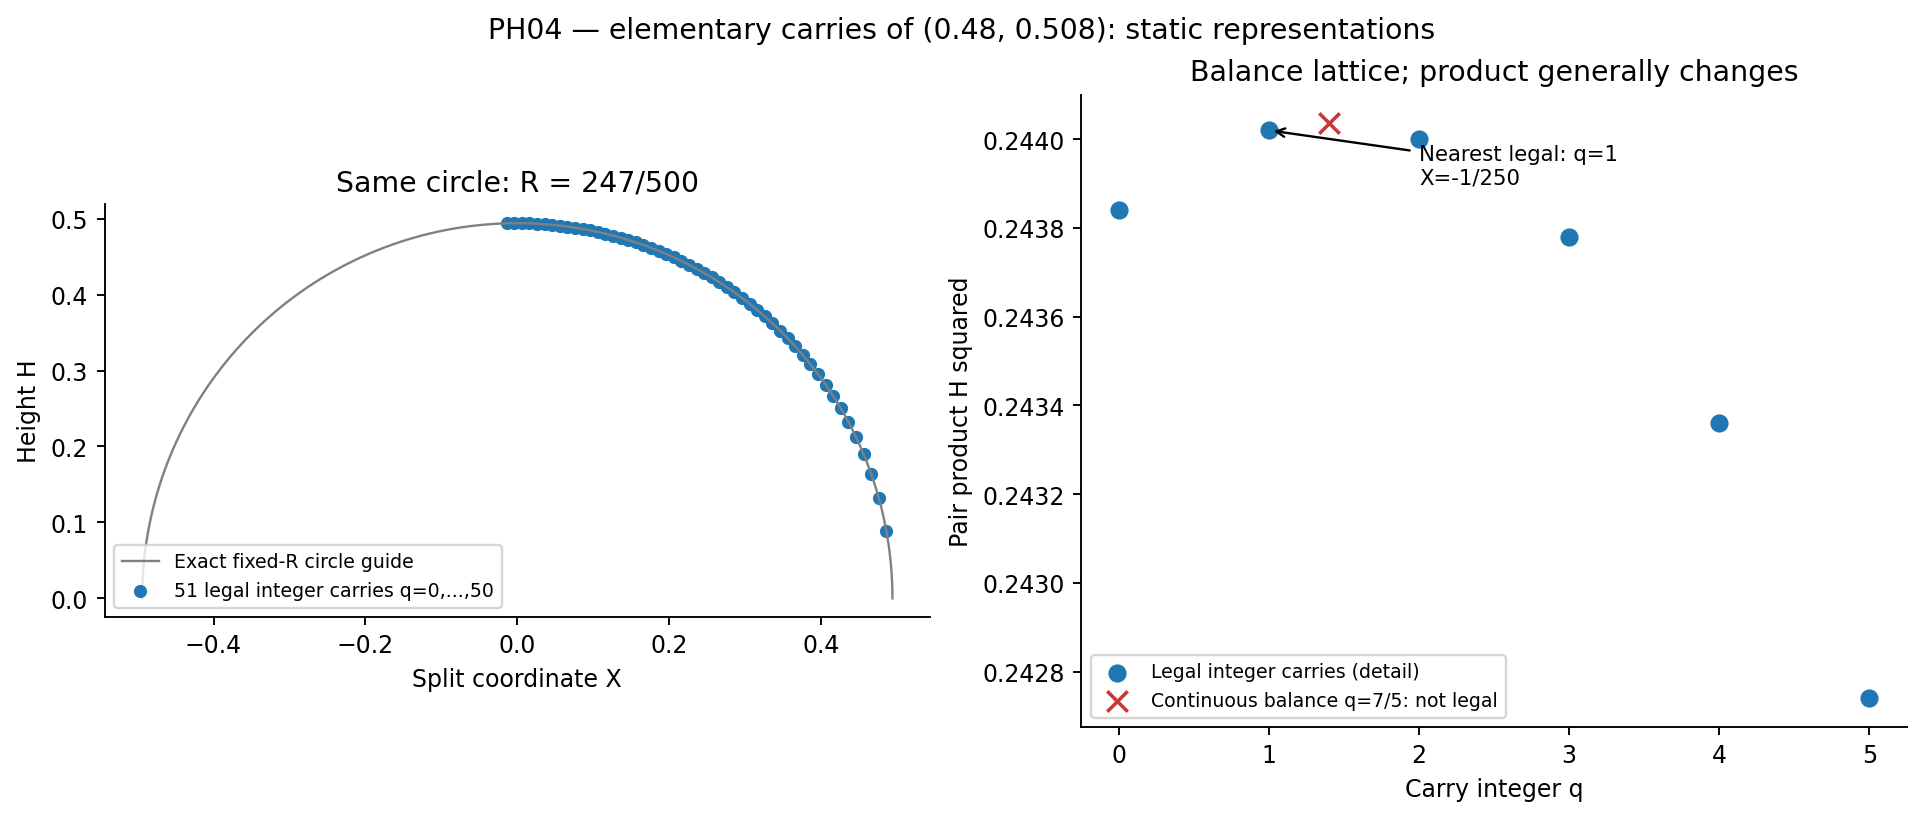
\includegraphics[width=\linewidth]{03_legal_carry_circle.png}
\caption{The accepted anchor carry figure, copied unchanged. The circle in the $(X,H)$ plane has fixed $R=247/500$. The right panel shows the legal integer lattice near balance; the continuous $q=7/5$ marker is explicitly not legal. The changing squared height is the changing pair product.}
\label{fig:carry}
\end{figure}
\finishwidepage

The inherited reciprocal action~\cite{ph03,multiplication} takes
\begin{equation}
(a,b)\mapsto(\lambda a,b/\lambda),\qquad \lambda>0,
\quad t=\log\lambda.
\label{eq:reciprocal}
\end{equation}
Adding and subtracting the new lengths yields
\begin{equation}
\binom{R'}{X'}=B(t)\binom RX,\qquad
B(t)=\begin{pmatrix}\cosh t&\sinh t\\\sinh t&\cosh t\end{pmatrix}.
\label{eq:B}
\end{equation}
Direct multiplication proves $B(t)^{\tr}JB(t)=J$ for $J=\diag(1,-1)$. It fixes $H^2=ab$ and stays on the future hyperbola in the $(R,X)$ plane. It generally changes R. This plus-sinh matrix is the active convention; no passive physical frame is assumed.

Choosing $\lambda=\sqrt{b/a}$ gives both new lengths equal to H. Hence $X'=0$ and $R'=H$. For the anchor the balanced subtotal becomes $2\sqrt{0.24384}$, while its product remains .24384. An integer carry instead retains subtotal .988 and generally changes that product. A fixed-radius circle in $(X,H)$ and a fixed-product hyperbola in $(R,X)$ are different loci in different coordinate planes.

The reciprocal balanced zero is deliberately selected. It is an auxiliary representation, never an unexpected cancellation found in the raw profile. Likewise the continuous optimum in Figure~\ref{fig:carry} does not enlarge the legal carry lattice.

\clearpage
\subsection{A full carry cascade exchanges value with other layers}
\label{sec:fullcarry}
The complete saved Q4 carry trace~\cite[Section 2]{ph02} illustrates why the isolated-pair result does not apply unchanged to a whole cascade. Value can enter or leave the chosen pair through its neighbors.

\begin{table}[ht]
\centering\small
\begin{tabular}{@{}p{.56\linewidth}rr@{}}
\toprule
Event at depths 2 and 3 & External change & Subtotal\\\midrule
Initial raw pair $(.48,.508)$ & --- & .988\\
Depth 4 sends coefficient 212 into depth 3 & $+.212$ & 1.200\\
Augmented internal carry $q=72$ at depth 3 & 0 & 1.200\\
Depth 2 sends coefficient 12 into depth 1 & $-1.200$ & 0\\\bottomrule
\end{tabular}
\caption{Saved full-carry accounting. The internal transfer is .720; it changes the two lengths but not their subtotal.}
\label{tab:fullcarry}
\end{table}
In pair coordinates, the successive representations are
\begin{equation}
(.48,.508)\longrightarrow(.48,.720)
\longrightarrow(1.200,0)\longrightarrow(0,0).
\label{eq:fullcarry}
\end{equation}
The internal $q=72$ is legal only after the incoming contribution raises coefficient 508 to 720. It is not a member of the original isolated $q=0,\ldots,50$ problem. The complete product remains
\begin{equation}
Q_4=1.2006509419262600.
\label{eq:Q4}
\end{equation}
Its depth 2 and depth 3 canonical digits are zero because value was carried to other depths, not because the scalar product disappeared. The complete lower-depth trace is retained in the exact-table supplement. For example, at depth 10 the raw coefficient 18096 receives carry 1313, giving total 19409, digit 9 and outgoing carry 1940. The saved JSON trace ends at depth 1; its last carry supplies the separately retained depth 0 digit 1.

The three operations can now be distinguished precisely:
\begin{center}\small
\begin{tabular}{@{}p{.29\linewidth}p{.30\linewidth}p{.32\linewidth}@{}}
\toprule
Operation & Preserved locally & What may change\\\midrule
Isolated elementary carry & $a+b=2R$ & $ab=H^2$, normalized split\\
Reciprocal scaling & $ab=H^2$ & $a+b=2R$, normalized split\\
Full canonical cascade & Complete weighted scalar total & Chosen pair subtotal and product\\\bottomrule
\end{tabular}
\end{center}
None specifies a physical history. Full carrying is a bookkeeping convention with a stated processing order, not an intrinsic time flow of the source multiplication.

\subsection{Zero cases and their domains}\label{sec:zeros}
For $(0,0)$, $R=X=H=0$, but x, y and rho are undefined. It is not a balanced \emph{positive} pair. With exactly one zero, $H=0$ and $(x,y)=(\pm1,0)$, but logarithmic and reciprocal formulas are undefined. Saved tables use null for undefined quantities, rather than infinities in ordinary arithmetic. All normalization and logarithmic theorems below explicitly require positive inputs; a run of positive layers ends at a zero rather than skipping over it.

\clearpage
\section{Moving from one pair to the next}
\label{sec:neighbor}
Let $a=w_k,b=w_{k+1},c=w_{k+2}$ be strictly positive. The first pair is $(a,b)$ and the next is $(b,c)$. Their heights and logarithmic coordinates satisfy
\begin{equation}
s_k=\frac{H_{k+1}}{H_k}=\sqrt{\frac ca},\qquad
\eta_k=\rho_{k+1}-\rho_k=\frac12\log\frac{b^2}{ac}.
\label{eq:s_eta}
\end{equation}

\begin{theorem}[Scale plus reciprocal action]
On every such positive triple,
\begin{equation}
\binom{R_{k+1}}{X_{k+1}}
=s_k B(\eta_k)\binom{R_k}{X_k}
=M_k\binom{R_k}{X_k},
\label{eq:interpair}
\end{equation}
where the complete scaled matrix is rational in the weights:
\begin{equation}
M_k=\frac12\begin{pmatrix}b/a+c/b&b/a-c/b\\b/a-c/b&b/a+c/b\end{pmatrix}.
\label{eq:M}
\end{equation}
It obeys
\begin{equation}
\det M_k=\frac ca,\qquad M_k^{\tr}JM_k=\frac ca J,
\qquad \frac{H_{k+1}^2}{H_k^2}=\frac ca.
\label{eq:bilinear}
\end{equation}
It is a pure fixed-invariant reciprocal action if and only if $c=a$, and a pure common positive scaling if and only if $b^2=ac$.
\end{theorem}
\begin{proof}
The height ratio follows from $H_k^2=ab$ and $H_{k+1}^2=bc$. Subtract the two logarithms to obtain eta. Positivity fixes the square-root branches and gives
\[
s_ke^{\eta_k}=b/a,\qquad s_ke^{-\eta_k}=c/b.
\]
Taking half-sums and half-differences yields the entries of~\eqref{eq:M}. In the coordinates $(R+X,R-X)=(a,b)$, its diagonal multipliers are $b/a$ and $c/b$. Thus it maps $(a,b)$ exactly to $(b,c)$, proving~\eqref{eq:interpair}.

Put $u=b/a,v=c/b$. The diagonal and off-diagonal entries of M are $(u+v)/2$ and $(u-v)/2$. Their squared difference is $uv=c/a$. Direct matrix multiplication then gives both the determinant and bilinear identity. The height ratio gives the last identity in~\eqref{eq:bilinear} as well.

A pure reciprocal action has $s=1$, which by positivity is equivalent to $c=a$. A pure common scaling has $\eta=0$, equivalently $b^2=ac$. These conditions are sufficient by the displayed decomposition and necessary by the positive height ratio and logarithmic coordinate, respectively.
\end{proof}
The result is valid for an arbitrary positive profile, without a decimal expansion or special constants. The SRG product supplies its particular inputs and invariant ratios. It does not provide a new general group law exclusive to SRG, and k is not being introduced as physical time.

\clearpage
\subsection{The actual first transition and a telescoping coordinate}
\label{sec:telescoping}
For the certified triple in~\eqref{eq:threeweights}, the accepted exact values are
\begin{equation}
s_2^2=\frac{71}{200},\quad
\eta_2=\frac12\log\frac{16129}{5112},\quad
M_2=\frac1{30480}\begin{pmatrix}21241&11017\\11017&21241\end{pmatrix}.
\label{eq:firstmatrix}
\end{equation}
Its local product changes from .24384 to .0865632, with ratio $71/200$. Describing this transition only as a fixed-product reciprocal action would omit that exact scale change. The saved displays give $s_2\approx0.595818764390649248$ and $\eta_2\approx0.574514088429905907$.

\begin{proposition}[Positive-block telescoping]
For a contiguous strictly positive block $w_r,\ldots,w_s$,
\begin{equation}
\sum_{k=r}^{s-1}\rho_k=\frac12\log\frac{w_r}{w_s}.
\label{eq:telescoping}
\end{equation}
For a singleton block the sum is empty and both sides are zero.
\end{proposition}
\begin{proof}
Add the logarithms $\rho_k=\tfrac12\log(w_k/w_{k+1})$. Their product of positive arguments telescopes to $w_r/w_s$. Positivity is needed for every logarithm; the statement cannot cross a zero layer.
\end{proof}

Eta has the sign of $b^2-ac$. For adjacent weighted raw coefficients the powers of ten cancel:
\begin{equation}
\frac{w_{k+1}^2}{w_kw_{k+2}}
=\frac{c_{k+1}^2}{c_kc_{k+2}}.
\label{eq:etasign}
\end{equation}
It compares the middle log weight with the average of its neighbors. It is the negative of half the usual second difference $\log w_k-2\log w_{k+1}+\log w_{k+2}$; it is not spacetime curvature.

There are certified examples in both directions. Equation~\eqref{eq:firstmatrix} has eta positive. The weights at depths 4, 5 and 6 give
\begin{equation}
(w_4,w_5,w_6)=\left(\frac{213}{1250},\frac{3429}{100000},\frac{7953}{1000000}\right),
\quad \frac{w_5^2}{w_4w_6}=\frac{1306449}{1505768}<1.
\label{eq:negativeeta}
\end{equation}
This eta is negative. Consequently the positive full raw region is neither everywhere log-concave nor everywhere log-convex. These are exact counterexamples, not extrapolations from a figure.

The finite Q64 certified triple set, $k=2,\ldots,62$, has 43 positive and 18 negative signs, with no zero. The complete finite Q64 raw set has 209 positive and 44 negative signs; those extra counts include finite tails. Across all 1,168 recorded positive triples there is no pure fixed-invariant reciprocal step. Ten carried triples have $\eta=0$ and are pure common scalings. These totals are finite observations from the saved evidence, not infinite frequencies or independent theorem counts.

\clearpage
\section{Two bounds with different meanings}
\label{sec:bounds}
\begin{theorem}[Unique global raw maximum]
For the fixed four-factor decimal product, $w_3=0.508$ is the unique largest full raw contribution over all depths.
\end{theorem}
\begin{proof}
The certified prefix through depth 6 is
\begin{equation}
(w_0,\ldots,w_6)=(0,0,.48,.508,.1704,.03429,.007953).
\label{eq:peakprefix}
\end{equation}
Its unique maximum is at depth 3. For any k there are $\binom{k+3}{3}$ weak compositions into four nonnegative indices, and every digit product is at most $9^4$. Therefore
\begin{equation}
0\le w_k\le U_k=9^4\binom{k+3}{3}10^{-k}.
\label{eq:U}
\end{equation}
At $k=7$ the upper bound is $U_7=.078732<.508$. Moreover
\begin{equation}
\frac{U_{k+1}}{U_k}=\frac{k+4}{10(k+1)}<1\qquad(k\ge7).
\label{eq:Uratio}
\end{equation}
Every later weight is therefore also less than .508. Together with the finite prefix, this proves uniqueness over every depth.
\end{proof}
This is a global size theorem from a finite prefix and a uniform tail bound. It is neither global monotonicity nor a theorem about globally nearest \emph{relative} balance. Two very small late weights could be close to one another without approaching the largest contribution.

\begin{theorem}[Canonical adjacent imbalance]
If u,v are positive canonical decimal digits at adjacent depths, then their normalized weighted imbalance satisfies
\begin{equation}
x=\frac{10u-v}{10u+v}\ge\frac1{19},
\qquad u,v\in\{1,\ldots,9\}.
\label{eq:canonicalbound}
\end{equation}
Equality holds exactly for $u=1,v=9$.
\end{theorem}
\begin{proof}
The weighted lengths are $a=u10^{-k}$ and $b=v10^{-(k+1)}$. Substitute them into~\eqref{eq:normalized}. Since $t=v/(10u)\le9/10$, and $(1-t)/(1+t)$ is strictly decreasing for positive t, the minimum is $(1-9/10)/(1+9/10)=1/19$. The bound on t is attained only for $u=1,v=9$.
\end{proof}
The raw anchor satisfies $7/247<1/19$, so it is closer to relative balance than any positive canonical adjacent decimal pair. Canonical digit pairs cannot attain the threshold $1/20$, much less exact balance. This conclusion is a general consequence of decimal weighting, not a special property of pi or zeta. It does not apply to arbitrary raw coefficients, negative inputs, or a pair selected by skipping zero gaps. The zero cases remain those of Section~\ref{sec:zeros}.

\clearpage
\section{The saved finite evidence and its populations}
\label{sec:scan}
The accepted arithmetic used exactly
\begin{equation}
d\in\{2,4,6,8,12,20,32,64\}.
\label{eq:schedule}
\end{equation}
The three earlier Q profiles at $d=2,4,6$ were reused from saved PH02 data. Five larger Q profiles and the single raw P64 control were new PH04 arithmetic. P64 is an adjacent-only three-factor control, not a statistical null ensemble. Q raw lags 2 and 3 are separate secondary comparisons; all Q carried pairs are adjacent finite-product output. No zero layer is skipped and silently renamed adjacent.

\begin{table}[ht]
\centering\small
\begin{tabular}{@{}lrrrr@{}}\toprule
Population & Rows & Positive & Left zero & Right zero / both\\\midrule
Q raw lag 1 & 592 & 573 & 8 & 3 / 8\\
Q raw lag 2 & 584 & 565 & 16 & 3 / 0\\
Q raw lag 3 & 576 & 557 & 16 & 3 / 0\\
Q carried lag 1 & 592 & 464 & 60 & 64 / 4\\
P64 raw lag 1 & 192 & 192 & 0 & 0 / 0\\\midrule
Total & 2536 & 2351 & 100 & 73 / 12\\\bottomrule
\end{tabular}
\caption{Complete declared finite populations. Zero domains are not positive balance. The table is transcribed from saved records; repeated prefixes and overlapping pairs are not independent samples.}
\label{tab:populations}
\end{table}

\begin{table}[ht]
\centering\small
\begin{tabular}{@{}lrp{.54\linewidth}@{}}\toprule
Status & Rows & Meaning\\\midrule
Certified raw prefix & 484 & Pair's largest depth is at most input precision d.\\
Finite raw tail & 1460 & Exact finite-product pair, without that sufficient full-profile guarantee.\\
Finite carried output & 592 & Raw-prefix theorem is inapplicable; canonical form of a finite product.\\\bottomrule
\end{tabular}
\caption{Certification is a separate classification from positivity and lag. These three groups partition the 2,536 rows.}
\label{tab:status}
\end{table}

No positive row in the declared scan has exact $X=0$. This finite finding is not a full-profile absence theorem. The raw leading $c_0,c_1$ zeros are exact because gamma starts with two zero digits. Three finite tail zeros are proved truncation-induced: Q4 depth 16 has a positive witness in Q6, Q20 depth 80 in Q32, and Q32 depth 128 in Q64. A positive later finite witness suffices, by nonnegativity, to prove positivity of the full coefficient; the entire witness tail need not itself be certified.

Raw profiles retain depths 0 through $4d$, including trailing zero coefficients. Their exact records contain 793 raw and 600 carried layer rows across the declared products, 77 contiguous positive blocks and 1,168 positive triples. The seven frozen JSON files preserve every pair, not only minima. Their archive and schema are described in Section~\ref{sec:data}.

\clearpage
\subsection{Finite ranks, relative scale, and separate controls}
\label{sec:ranks}
Ranking uses the exact rational $|x|$, not a small absolute X. Every saved rank retains the pair subtotal and support $(a+b)/Q_d$ or $(a+b)/P_d$. Exact ties receive competition ranks. Thresholds $1/1000,1/100,1/20$ are declared reporting choices, not universal constants or significance levels.

\begin{table}[ht]
\centering\small
\begin{tabular}{@{}rrrrll@{}}\toprule
$d$ & Rows & Positive & Cert. positive & Minimum $|x|$ & Counts at thresholds\\\midrule
2 & 8 & 6 & 0 & $1/119$, tail & 0 / 1 / 1\\
4 & 16 & 13 & 2 & $7/247$, prefix & 0 / 0 / 1\\
6 & 24 & 22 & 4 & $7/247$, prefix & 0 / 0 / 1\\
8 & 32 & 30 & 6 & $7/247$, prefix & 0 / 0 / 1\\
12 & 48 & 46 & 10 & $7/247$, prefix & 0 / 0 / 1\\
20 & 80 & 77 & 18 & $7/247$, prefix & 0 / 0 / 1\\
32 & 128 & 125 & 30 & $7/247$, prefix & 0 / 0 / 1\\
64 & 256 & 254 & 62 & $7/247$, prefix & 0 / 0 / 1\\\bottomrule
\end{tabular}
\caption{Q raw adjacent populations. Every minimum is at depths (2,3). Counts are positive-only and cumulative for $|x|\le.001,.01,.05$, in that order.}
\label{tab:ranks}
\end{table}
The specified Q64 certified adjacent positive population consists exactly of $(k,k+1)$ for $k=2,\ldots,63$. The anchor is uniquely rank 1 of 62. The next is (3,4), with $|x|=211/424$. The anchor's subtotal is exactly $247/250$, and its finite Q64 support is approximately .821924484109739. It is also first among the 254 positive adjacent rows of the complete finite Q64 profile, but that larger set includes truncated tails. Neither rank is a p-value or a globally closest-pair theorem.

All positive raw lag 2 and lag 3 rows lie outside $|x|\le1/20$ in the declared scan. Lag 2 minima occur at (2,4): $73/127$ in Q2, then $129/271$. Lag 3 minima occur at (2,5): $73/77$ in Q2, $119/137$ in Q4, then $14857/17143$ from Q6 onward. The Q4 lag 3 pair is a finite tail; its later value is fixed by common $d=5$, first present at scheduled $d=6$. No new intermediate precision was computed.

For carried positive pairs, the general bound in~\eqref{eq:canonicalbound} explains the zero counts at all three thresholds. The minimum observed across those populations is $1/19$, attained in Q4, Q8 and Q64. Endpoint and double-zero cases are excluded from positive ranks.

The sole P64 control has 192 positive adjacent pairs, of which 64 are certified raw-prefix pairs. Its closest pair is $(6,5.9)$ at depths (0,1), with $x=1/119$ and subtotal 11.9. It is the only control pair within .01 or .05, and none is within .001. The $d=2$ Q anchor is precisely these first two P layers multiplied by the sole retained gamma contribution .08 and shifted two depths. Gamma's next contribution changes the true Q geometry as proved in~\eqref{eq:omitted}. Control support is divided by P64, never by Q64.

\clearpage
\beginwidepage
\subsection{Views of the same saved profiles}
\label{sec:figures}
\begin{figure}[!ht]
\centering
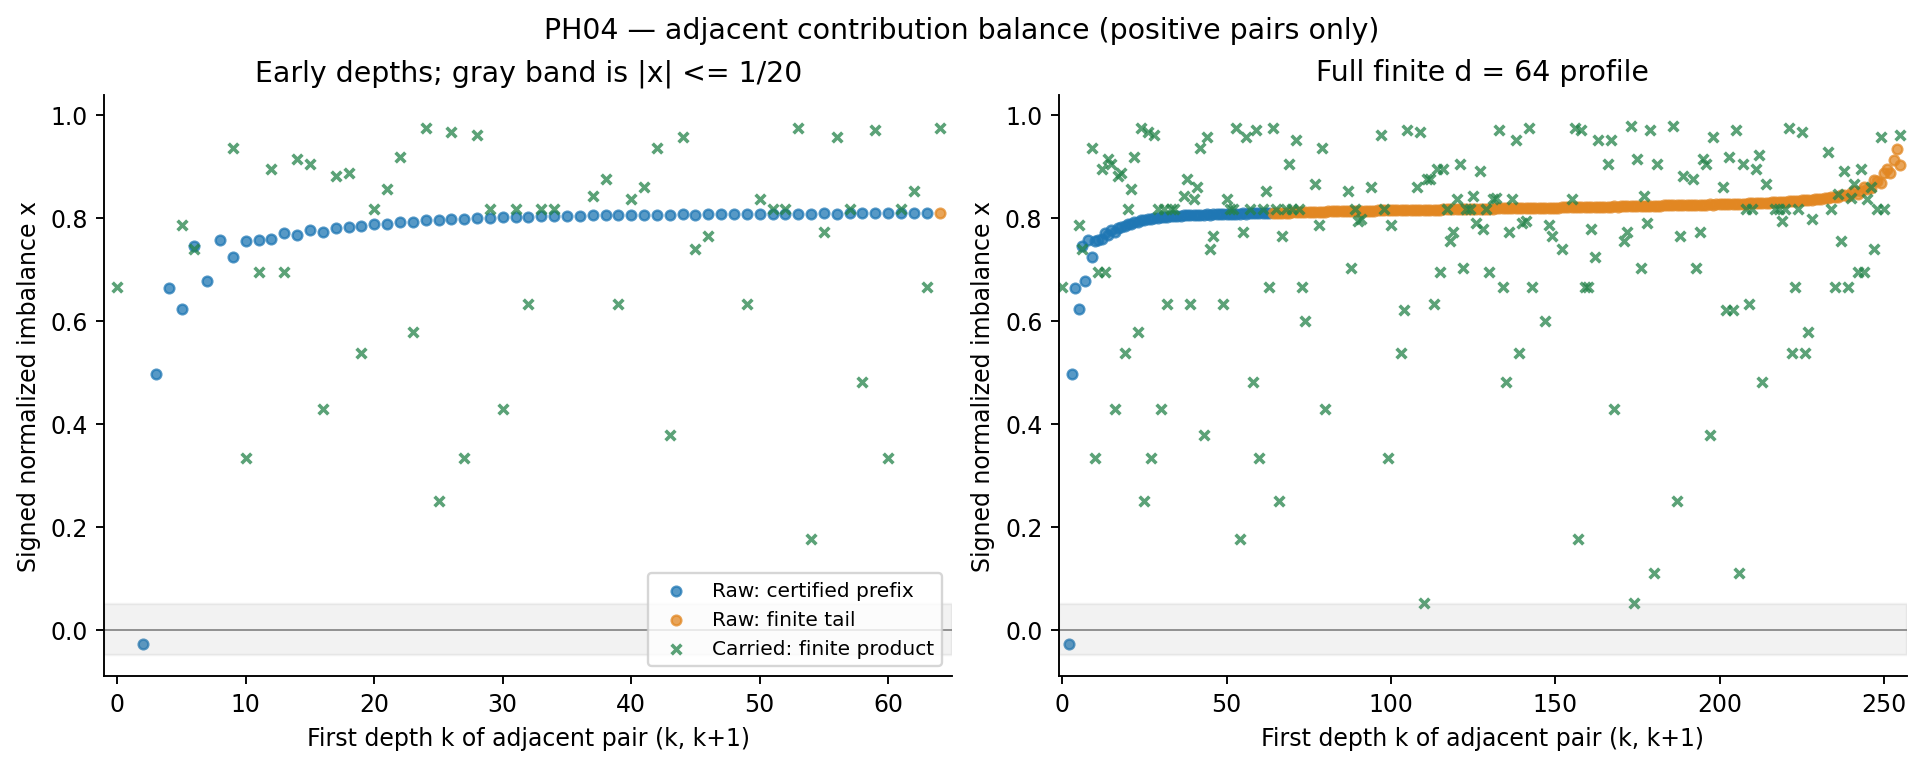
\includegraphics[width=\linewidth]{01_imbalance_by_depth.png}
\caption{Positive adjacent Q64 pairs. Blue points are certified raw-prefix pairs; orange points are exact finite-tail pairs; green crosses are finite carried-output pairs. The two panels show early and complete finite depths. The shaded band is the declared $|x|\le1/20$ threshold, not a statistical interval. The anchor's exact subtotal is .988 and its support is about .821924484109739 of Q64. No fitted law is shown.}
\label{fig:imbalance}
\end{figure}
\finishwidepage
\beginwidepage
\begin{figure}[!ht]
\centering
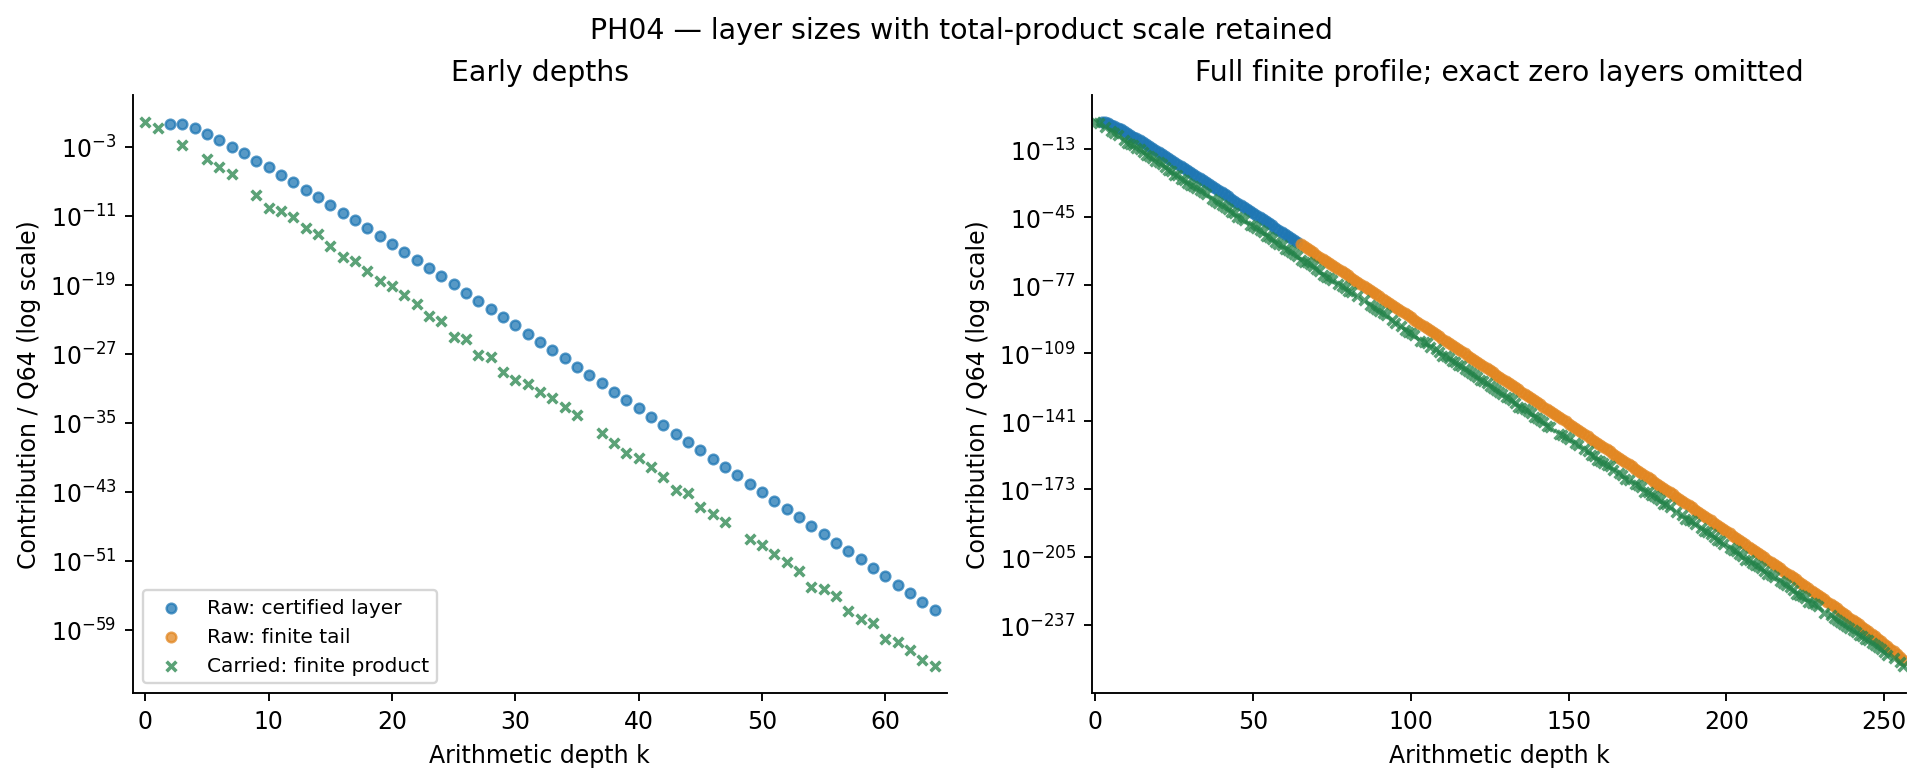
\includegraphics[width=\linewidth]{02_relative_contributions.png}
\caption{Layer weights divided by exact finite Q64, retaining scale beside the normalized view. Certified raw layers, raw finite tails and carried output have distinct colors and markers. Exact zero layers are omitted from logarithmic axes because log(0) is undefined; no artificial numerical floor replaces them. These plots are arithmetic illustrations, not particle trajectories.}
\label{fig:sizes}
\end{figure}
\finishwidepage
The accepted figure bytes are unchanged. Signs, exact balances and rankings come from rational tables. Dense points may overlap at rendering resolution; pixel coincidence does not establish algebraic equality. Small far-tail absolute X reflects small lengths and is not evidence of near-balance without the relative coordinate x.

\begin{figure}[ht]
\centering
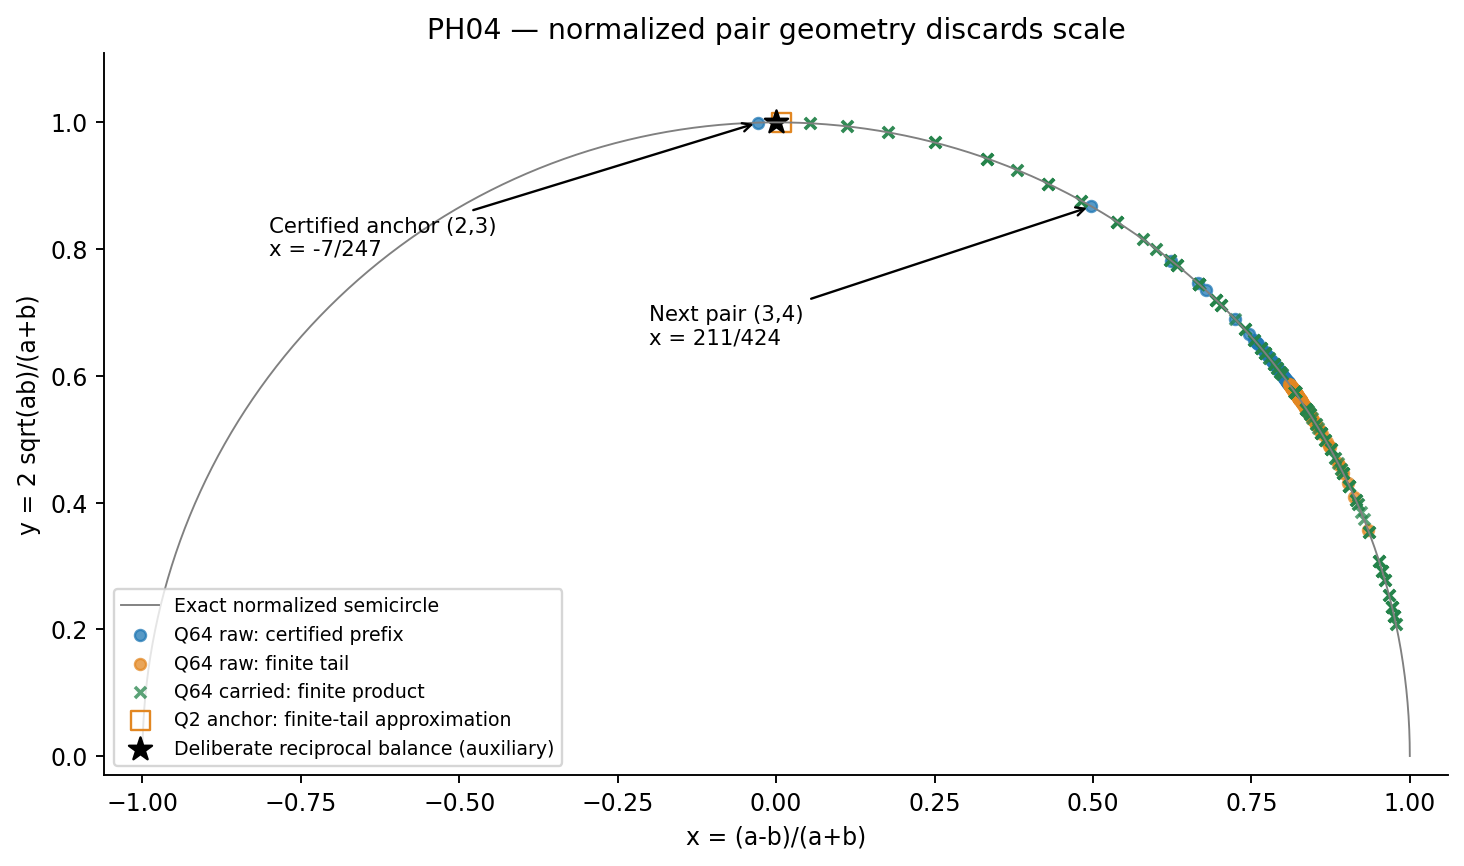
\includegraphics[width=.94\linewidth]{04_normalized_pair_geometry.png}
\caption{Normalized positive-pair geometry. Certified raw-prefix, finite-tail and finite carried-output points are distinct populations. The Q2 anchor is a finite approximation with the opposite sign from the permanent anchor. The black star is deliberately reciprocal-balanced, not an observed raw zero. Normalization removes the radius: the actual anchor has $R=.494$, the next pair $R=.3392$, and their squared heights are .24384 and .0865632. The reference semicircle is exact geometry, not a fit.}
\label{fig:normalized}
\end{figure}

\section{A conditional interpretation, without a new dynamic}
\label{sec:interpretation}
The inherited dictionary~\cite[Section 6]{ph03}, also developed in~\cite{multiplication}, introduces a positive energy scale K and reference speed c. With both held fixed, assign
\begin{equation}
E_{\rm cand}=KR,\qquad p_{\rm cand}=KX/c,\qquad
m_{\rm cand}=KH/c^2.
\label{eq:dictionary}
\end{equation}
Equation~\eqref{eq:circle} then gives the algebraic relation
\begin{equation}
E_{\rm cand}^2-c^2p_{\rm cand}^2=m_{\rm cand}^2c^4.
\label{eq:shell}
\end{equation}
This reuses the conditional correspondence; it does not independently derive the physical law or identify measured quantities. The original diagnostic reference is the PDG kinematics review~\cite{pdg}, previously inspected in PH03. No new physical-source review or calibration was performed here.

For neighboring pairs, fixed K,c imply $m_{{\rm cand},k+1}/m_{{\rm cand},k}=s_k$. Varying H therefore changes the represented invariant scale; it is not a series of frame changes of one fixed measured mass. Neither the carry product .24402 nor the next product .0865632 is fitted to a source constant. The digit weights supply no physical clock, propagation law, measured energy, photon identification or invariant speed. The geometric results stand independently of such assignments.

\clearpage
\appendix
\section{Certification of the saved input digits}
\label{app:cert}
This appendix supplies the proofs behind the accepted rational brackets; manuscript preparation transcribes their saved values and does not recompute them. PH04 used one common 100-place internal target, within its 160-place limit, and all 32 factor/precision floors resolved. Display precision alone would not certify them.

For $0<z<1$, an alternating arctan sum lies between its partial sum and that sum plus its next signed term. The Machin identity is
\begin{equation}
\pi=16\arctan(1/5)-4\arctan(1/239).
\label{eq:machin}
\end{equation}
To fix its branch, put $u=\arctan(1/5)$. The tangent doubling formula gives $\tan2u=5/12$ and $\tan4u=120/119$. Subtraction of $\arctan(1/239)$ gives tangent 1. The angle is positive and less than .8, hence in the first quadrant; it equals $\pi/4$. The recorded enclosures used 71 terms at 1/5 and 21 at 1/239. Negative coefficients in~\eqref{eq:machin} reverse the corresponding interval endpoints.

For e, start with $\sum_{j=0}^n1/j!$. After the first omitted term, each ratio is at most $1/(n+2)$, so its positive remainder is at most
\begin{equation}
T_n=\frac1{(n+1)!}\frac{n+2}{n+1}.
\label{eq:etail}
\end{equation}
The saved final index was $n=69$. For phi, let $D=10^{100}$ and let t be the integer square root of $5D^2$. The exact inequalities $t^2<5D^2<(t+1)^2$ give a containing bracket $t/D<\sqrt5<(t+1)/D$. Apply $(1+\cdot)/2$ to both endpoints.

Multiplication of positive interval endpoints bounds P. With the zeta interval established in Appendix~\ref{app:zeta}, positivity gives
\begin{equation}
\gamma\in\left[\frac{\zeta_L}{\pi_Ue_U\varphi_U},
\frac{\zeta_U}{\pi_Le_L\varphi_L}\right].
\label{eq:gammabounds}
\end{equation}
For each factor and each scheduled d, the saved certificate proves
\begin{equation}
\lfloor10^d f_L\rfloor=\lfloor10^d f_U\rfloor.
\label{eq:floors}
\end{equation}
The true floor lies between these equal integers. Exact rational endpoints and margins to the adjacent integers are included in the supplement, so this is stronger than agreement between two approximate evaluations.

Saved width displays are approximately $1.253\times10^{-101}$ for pi, $8.468\times10^{-101}$ for e, $5\times10^{-101}$ for phi, $7.620\times10^{-101}$ for zeta(3), $9.125\times10^{-100}$ for P, and $1.126\times10^{-101}$ for gamma. No internal escalation beyond 100 places was needed. Gamma's bracket comes from the exact relation, never a recalibration against finite $Q_d$.

\clearpage
\section{The accelerated zeta bracket: a complete proof}
\label{app:zeta}
Define the rational finite differences
\begin{equation}
A_k=\sum_{j=0}^k\frac{(-1)^j\binom kj}{(j+1)^3}.
\label{eq:Ak}
\end{equation}
The elementary integral $\int_0^1t^j\log^2t\,dt=2/(j+1)^3$, obtained by differentiating $1/(j+1)$ twice, and the binomial expansion give
\begin{equation}
A_k=\frac12\int_0^1\log^2t(1-t)^k\,dt,
\qquad 0<A_k\le1.
\label{eq:Akint}
\end{equation}
The upper bound follows from $(1-t)^k\le1$. For the efficient harmonic form, use
\[
B(\alpha,k+1)=\int_0^1t^{\alpha-1}(1-t)^k\,dt
=\frac{k!}{\alpha(\alpha+1)\cdots(\alpha+k)}.
\]
The product formula follows by integration by parts, beginning with $B(\alpha,1)=1/\alpha$. Differentiate twice at $\alpha=1$. On a compact positive-alpha neighborhood, an integrable power of t times $|\log t|^2$ justifies differentiation under the integral. Logarithmic differentiation of the product, with $n=k+1$, gives
\begin{equation}
A_k=\frac{\mathcal H_{k+1}^2+\mathcal H_{k+1}^{(2)}}{2(k+1)},\qquad
\mathcal H_n=\sum_{j=1}^n\frac1j,\quad
\mathcal H_n^{(2)}=\sum_{j=1}^n\frac1{j^2}.
\label{eq:harmonic}
\end{equation}
Indeed $B(1,k+1)=1/n$, the first logarithmic derivative is $-\mathcal H_n$, and the second is $\mathcal H_n^{(2)}$. These harmonic sums are distinct from circle height H. PH04 independently compared the two rational formulas for $k=0,\ldots,16$; generality comes from this proof, not those finite checks.

All integrands in~\eqref{eq:Akint} are nonnegative. Monotone convergence and the geometric series therefore imply
\begin{equation}
\sum_{k=0}^{\infty}\frac{A_k}{2^{k+1}}
=\frac12\int_0^1\frac{\log^2t}{1+t}\,dt
=\sum_{n=1}^{\infty}\frac{(-1)^{n-1}}{n^3}
=\frac34\zeta(3).
\label{eq:zetaseries}
\end{equation}
The middle equality follows from finite geometric expansions and dominated convergence, or absolute summability of integrated term magnitudes. Separating even terms in the absolutely convergent zeta series gives the factor $1-2/2^3=3/4$. Finally $A_k\le1$ bounds the omitted geometric tail:
\begin{equation}
0\le\zeta(3)-\frac43\sum_{k=0}^{N-1}\frac{A_k}{2^{k+1}}
\le\frac43\,2^{-N}.
\label{eq:zetatail}
\end{equation}
The accepted computation used 333 rational terms and this explicit remainder. The method is arithmetic support, not an added SRG operator or a new scan. No root, logarithm, bracket or coefficient was recalculated for this manuscript.

\clearpage
\section{Evidence, reproducibility and the remaining question}
\label{sec:data}
The proposed public supplement \texttt{SRG\_PH04\_EXACT\_TABLES\_v0.1.zip} contains exactly seven original PH04 JSON files, unchanged at their archive root:
\begin{center}\small
\begin{tabular}{@{}lp{.54\linewidth}@{}}\toprule
File & Role\\\midrule
\texttt{constant\_certificates.json} & Rational bounds, floor certificates and display conventions\\
\texttt{profiles.json} & Full factor arrays, raw/carried coefficients and exact weights\\
\texttt{pairs.json} & All labelled pairs, exact geometry, domains and support\\
\texttt{triples\_and\_blocks.json} & Scaled matrices, sign arguments and contiguous blocks\\
\texttt{ranked\_summaries.json} & All 57 grouped rankings, ties, thresholds and scales\\
\texttt{anchor\_carries\_and\_terms.json} & All 51 carries, full saved trace and labelled terms\\
\texttt{findings.json} & Exact anchor, witnesses and accepted bound evidence\\\bottomrule
\end{tabular}
\end{center}
Fractions and integers are authoritative. Root/log display strings were saved using 100 decimal working places and 24 significant-digit formatting; undefined values are null. The reader-facing data guide maps retained references to the original PH04 \texttt{REPORT.md} onto this paper's section/equation locators. Frozen JSON locators are not silently rewritten. The new archive changes packaging only.

The accepted execution compared finite convolution evaluation with direct integer products, canonical reconstruction with the same rational values, and certified prefixes across scheduled depths. It records 12 symbolic residuals and 10,664 repeated successful assertion evaluations, not independent theorems. Its first invocation stopped on a reader-format error: a nested \texttt{exact\_product} object was passed to Fraction instead of its \texttt{exact} scalar. That was not a mathematical counterexample. The failed script, command evidence and sole reader correction remain preserved privately. The completed result and GPT acceptance~\cite{review} are unchanged.

Preparation of this edition reused those accepted proofs, tables and figures. New work checked transcription, citations, labels, compilation, every rendered page and artifact identities. It did not execute any accepted checker, reviewer helper or historical program. Internal GPT acceptance of PH04 is not journal acceptance or external peer review; this new manuscript and its exact twelve-file payload await manuscript-and-payload review.

The exact-prefix theorem, carry lattice, full-carry distinction, interpair law and two global bounds support a coherent account of contribution geometry. One question remains deliberately open: does every positive full raw adjacent pair with k at least 64 satisfy $|x_k|>7/247$? The finite rank does not settle it, and no longer scan or proposed recurrence was undertaken here.

\paragraph{Authorship, assistance and reuse.}
Hilmir Frímann Halldórsson is the human author. GPT assisted with mathematical proposals and scientific review; Codex performed the accepted PH04 analysis and prepared this exposition, source records and artifact QA under the author's direction. These tools are not coauthors. This separate follow-on does not revise SRG-I, Origins, the preceding multiplication paper or the reserved SRG-II scope. No new blanket reuse licence is granted and software licensing is not extended to research; existing source-specific notices remain with their sources.

\clearpage
\begin{thebibliography}{9}
\bibitem{ph04}
H. F. Halldórsson, with GPT/Codex assistance, \emph{SRG-PH04: Geometry of neighboring decimal contributions}, accepted private report, 13 October 2026, Sections 1--8. Saved exact arithmetic, source ledger and four figures; precise file identities appear in the companion \texttt{SOURCE\_INDEX.md}. Its proofs are supplied in this paper and its seven exact tables in the proposed data supplement.
\bibitem{review}
GPT, \emph{Scientific review: PH04 neighboring contribution geometry}, 13 October 2026. Internal assisted scientific decision: accepted within declared exact-arithmetic and geometric scope, no required scientific revisions. Retained private decision, not external peer-reviewed literature. No review script was rerun in manuscript preparation.
\bibitem{ph02}
H. F. Halldórsson, with GPT/Codex assistance, \emph{SRG-PH02: Multiplication geometry}, accepted private report, 13 October 2026, Sections 2--3 and 5.1; saved \texttt{CHECK\_RESULTS.json}. Source of the labelled convolution, finite examples, carrying and convergence convention. Relevant original locators are retained in PH04's source excerpts and the companion source index.
\bibitem{ph03}
H. F. Halldórsson, with GPT/Codex assistance, \emph{SRG-PH03: From a split-diameter circle to a positive mass shell}, accepted private report, 13 October 2026, Sections 1--4 and 6. Source of the positive-pair inverse, reciprocal action, normalization limits and conditional dictionary, Eqs. (26)--(30) for the latter.
\bibitem{multiplication}
H. F. Halldórsson, \emph{SRG Multiplication Geometry: Factor Data, Circle Construction, and Mass-Shell Correspondence}, v0.1, 13 October 2026. Separate preceding manuscript. Local edition in \texttt{SRG\_REDISCOVERY/PAPERS/}\allowbreak\texttt{SRG\_MULTIPLICATION\_MASS\_SHELL/}\allowbreak\texttt{publication/v0.1/}. Its existing publication workflow and status were not rechecked or changed for this paper.
\bibitem{pdg}
Particle Data Group, \emph{Kinematics}, 2025 update, physical p.1, Section 49.1 and Eq. (49.1). \href{https://pdg.lbl.gov/2025/reviews/rpp2025-rev-kinematics.pdf}{Official PDG review PDF}. Original external diagnostic citation inherited from the accepted PH03 review; not newly downloaded or re-audited here. The conditional comparison does not turn the arithmetic depth index into time or assign a physical speed.
\end{thebibliography}
\end{document}
